\chapter*{Hasil}
\addcontentsline{toc}{chapter}{Hasil}

Kami melakukan uji coba model dengan skenario dataset yang memiliki total 33 fitur, dan fitur yang dipakai untuk memprediksi kinerja akademik siswa. Fitur-fitur tersebut 
meliputi nilai ujian sebelumnya {(G1, G2, dan rata-ratanya)}, data demografi dan keluarga {(usia, pendidikan orang tua, jenis kelamin, alamat)}, 
serta kebiasaan belajar dan sekolah (waktu belajar, kegagalan sebelumnya, absensi, akses internet, partisipasi kegiatan). Kami juga menyertakan 
aspek gaya hidup dan sosial siswa, seperti frekuensi bersosialisasi, status kesehatan, status hubungan romantis, dan konsumsi alkohol, dengan jumlah
siswa total 395.
Setelah melakukan uji coba didapatkan hasil sebagai berikut

\section{Uji Coba dengan Data Siswa}

\begin{figure}[h]
    \centering
    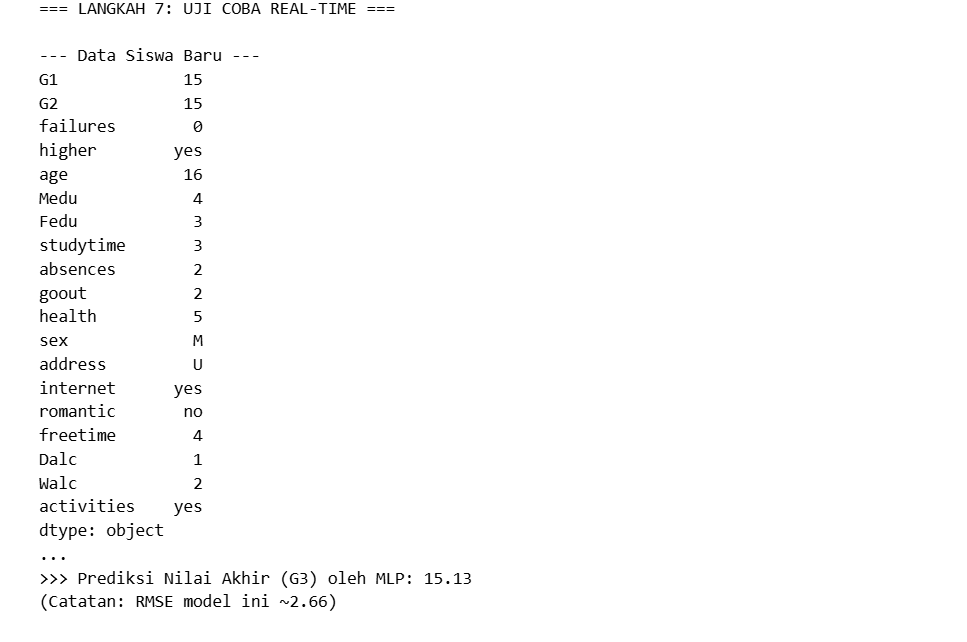
\includegraphics[width=0.8\textwidth]{images/datasiswa2.png}
    \caption{Data Siswa Pertama}
    \label{fig:datasiswa1}
\end{figure}

Di sini pada nilai aktualnya nilai G3 siswa adalah 15, dan saat dilakukan uji coba prediksi didapatkan setiap model seperti yang ada 
pada gambar berikut.

\begin{figure}[h]
    \centering
    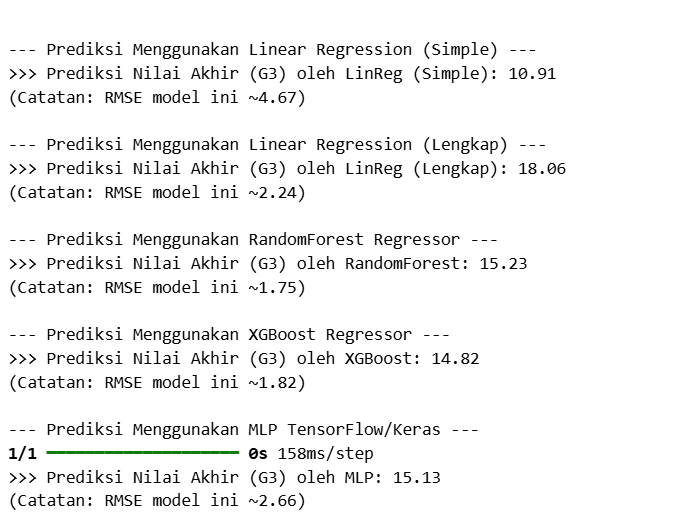
\includegraphics[width=0.8\textwidth]{images/hasil2.png}
    \caption{Hasil Uji Coba Model Pertama}
    \label{fig:hasil1}
\end{figure}

Dilanjutkan uji coba dengan data siswa sebagai berikut:

\begin{figure}[h]
    \centering
    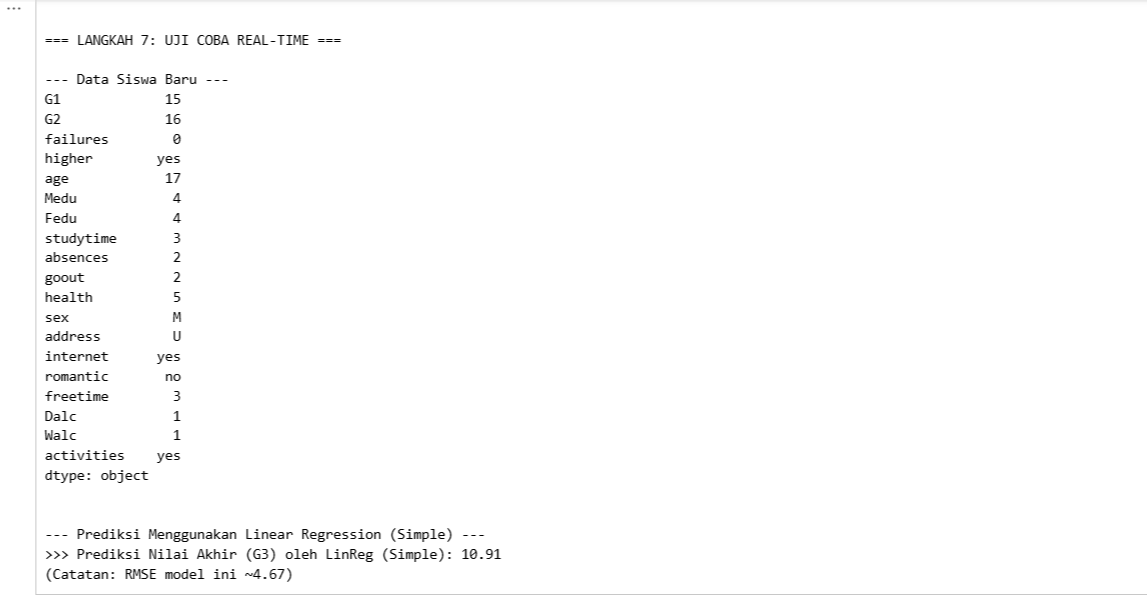
\includegraphics[width=0.8\textwidth]{images/datasiswa1.png}
    \caption{Data Siswa Kedua}
    \label{fig:datasiswa2}
\end{figure}

Dengan data siswa tersebut, kami mengasumsikan bahwa siswa tersebut memiliki nilai G3 sebesar 14,5 yang didapat dengan perkiraan secara 
intuitif menggunakan heatmap yang ada dan didapatkan hasil seperti pada gambar berikut.

\begin{figure}[h]
    \centering
    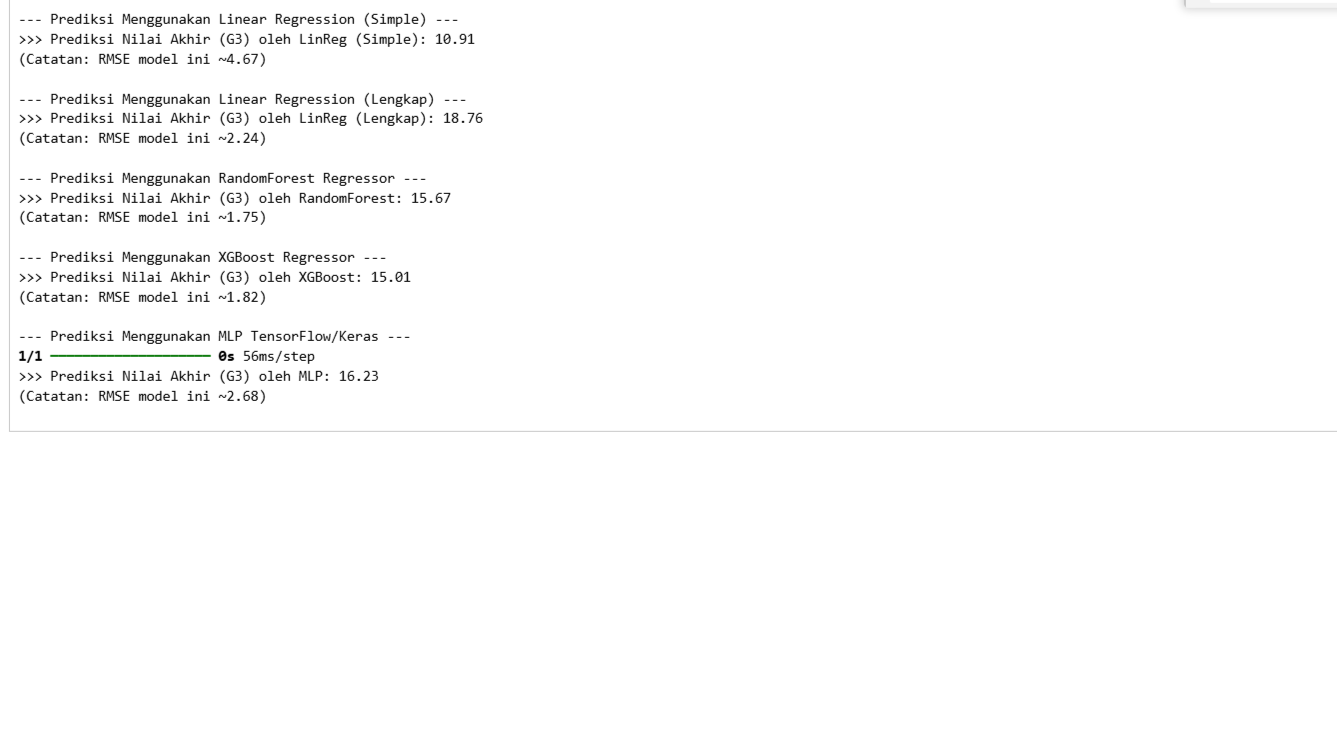
\includegraphics[width=0.8\textwidth]{images/hasil1.png}
    \caption{Hasil Uji Coba Model Kedua}
    \label{fig:hasil2}
\end{figure}

\section{Evaluasi Model}

Berikut adalah visualisasi untuk RMSE (Root Mean Square Error) dan R-Squared, di mana nilai RMSE yang baik adalah mendekati 0 dan R-Squared 
mendekati 1.

\begin{figure}[h]
    \centering
    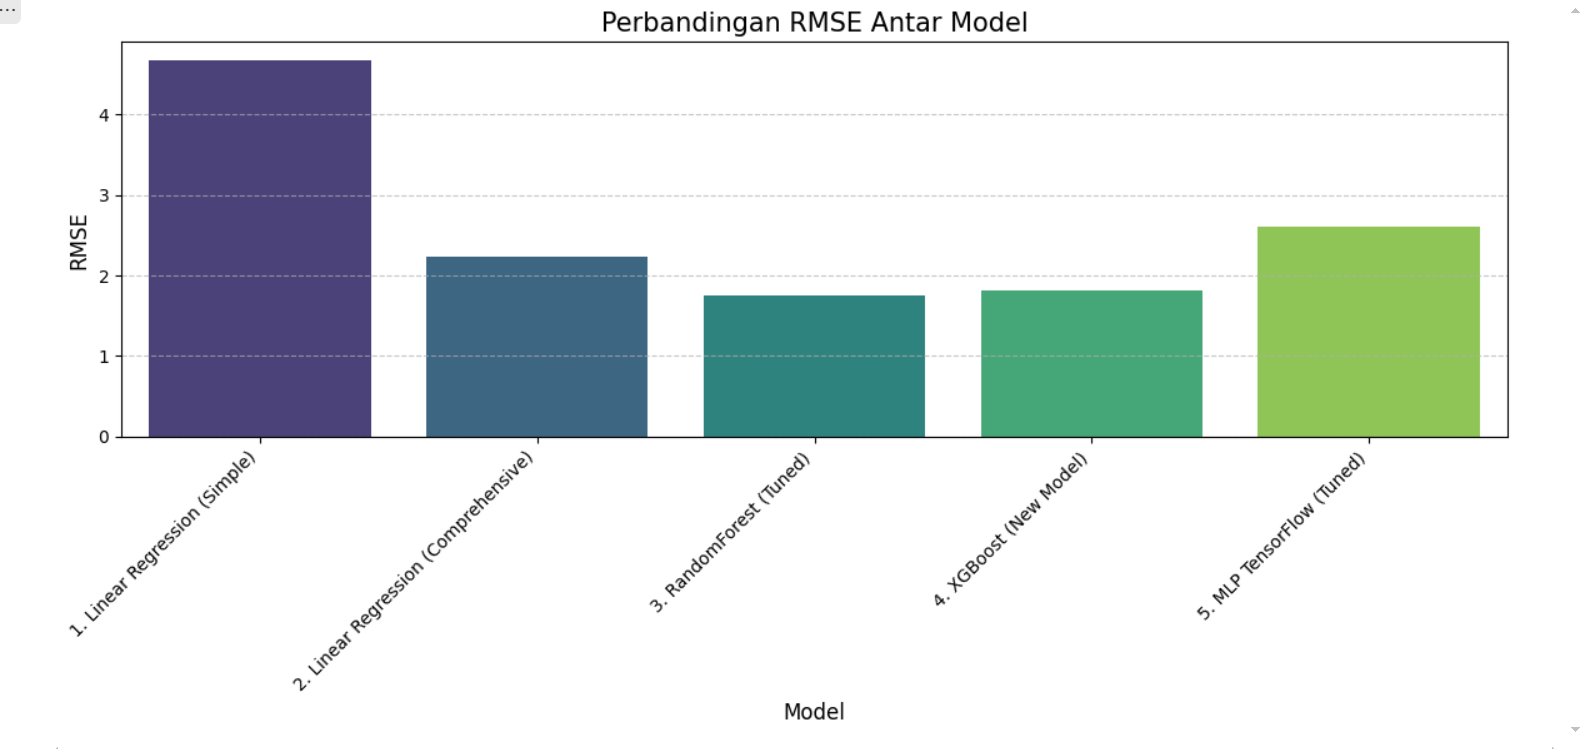
\includegraphics[width=0.8\textwidth]{images/rmse.png}
    \caption{Visualisasi RMSE}
    \label{fig:rmse}
\end{figure}

\begin{figure}[h]
    \centering
    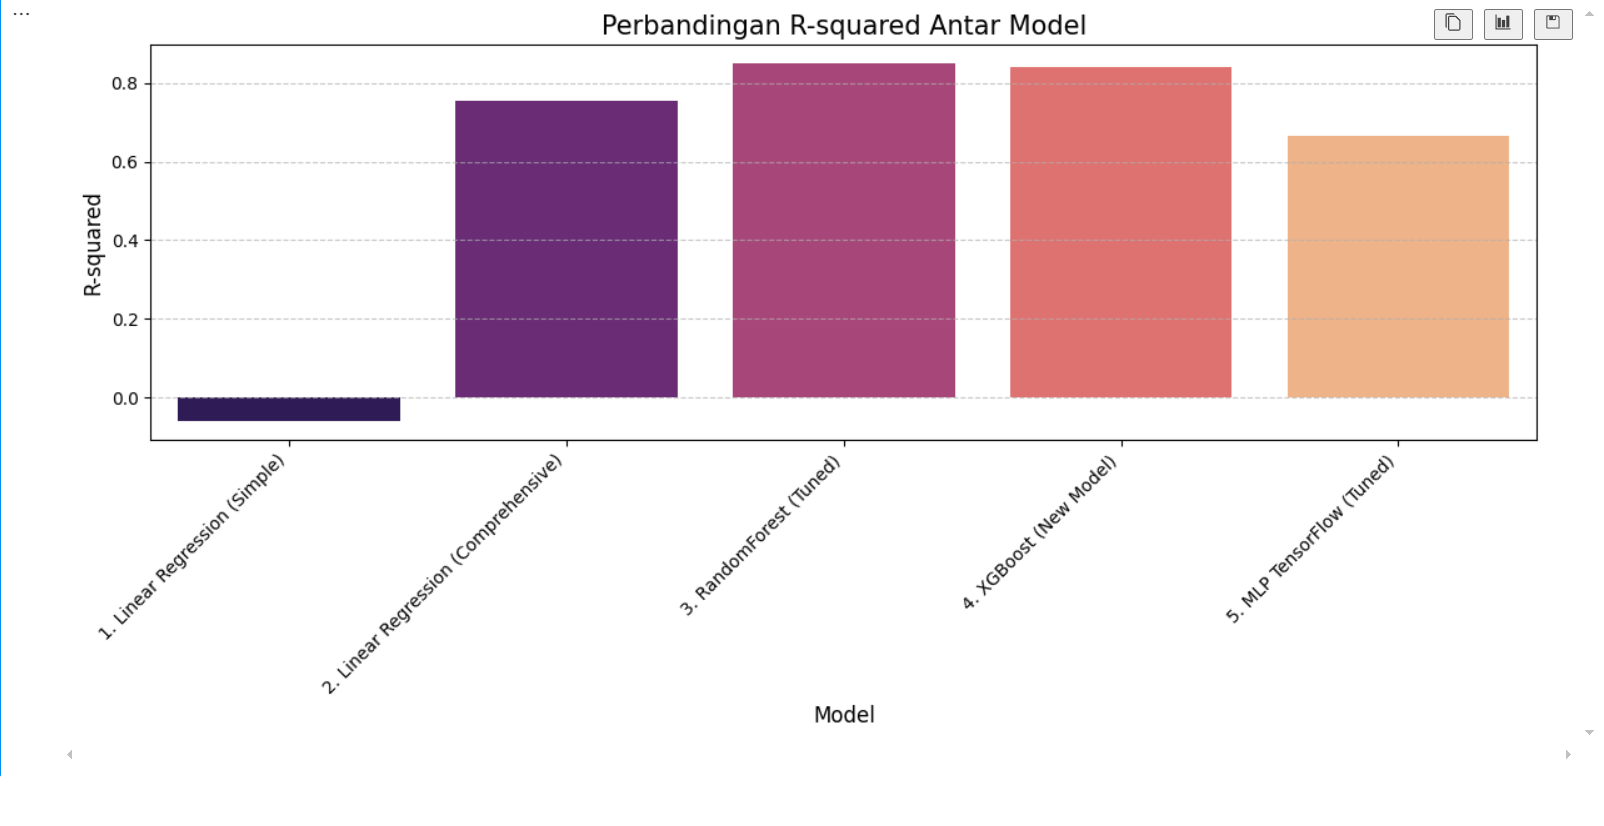
\includegraphics[width=0.8\textwidth]{images/r-squared.png}
    \caption{Visualisasi R-Squared}
    \label{fig:rsquared}
\end{figure}

Dari data tersebut RandomForest Regressor mendapatkan nilai RMSE yang lebih rendah daripada semua model yang ada, diikuti oleh XGBoost, 
Linear Regression dengan fitur yang lengkap, lalu MLP TensorFlow. Nilai RMSE menunjukkan berapa rentang error yang dihasilkan oleh data. 
Untuk R-Squared, RandomForest Regressor juga merupakan yang paling baik di antara model yang ada. R-Squared menunjukkan informasi mengenai 
bagaimana model tersebut menjelaskan variabilitas data terhadap model yang digunakan. R-Squared menggambarkan seberapa baik model sesuai 
dengan data yang digunakan.

Secara teknis, RandomForest Regressor mungkin lebih cocok untuk dataset yang relatif lebih kecil dibandingkan MLP TensorFlow dan XGBoost. 
RandomForest umumnya dianggap lebih tidak rumit dalam interpretasi dan implementasi dibandingkan dua model lainnya.

Dapat dilihat bahwa performa model RandomForest Regressor adalah model dengan prediksi yang paling akurat dibandingkan dengan model-model lain. 
Hal ini dapat terjadi dikarenakan RandomForest Regressor merupakan model yang memang cocok untuk dataset yang lebih kecil daripada MLP TensorFlow 
dan XGBoost. Jika dibandingkan secara teknis, RandomForest merupakan model yang paling tidak rumit dibanding dua model tersebut. RandomForest 
Regressor bekerja dengan membuat decision tree secara paralel dengan memilih data secara acak, dan dari decision tree yang sudah dibuat secara 
paralel nilai prediksi dari setiap decision tree tersebut akan dirata-rata untuk mendapatkan hasilnya. XGBoost juga masih menggunakan decision 
tree, namun dengan cara memperbaiki kesalahan berulang kali dari decision tree sebelumnya. Untuk penjelasan simpelnya, MLP TensorFlow sendiri 
merupakan salah satu model jaringan saraf tiruan yang memiliki tiga komponen, yaitu \textit{Input Layer}, \textit{Hidden Layer}, 
dan \textit{Output Layer} yang memiliki cara pemodelan yang lebih kompleks dibandingkan RandomForest Regressor dan XGBoost.

\section{Visualisasi Scatter Plot}

Kami juga melakukan visualisasi menggunakan scatter plot.

\begin{figure}[h]
    \centering
    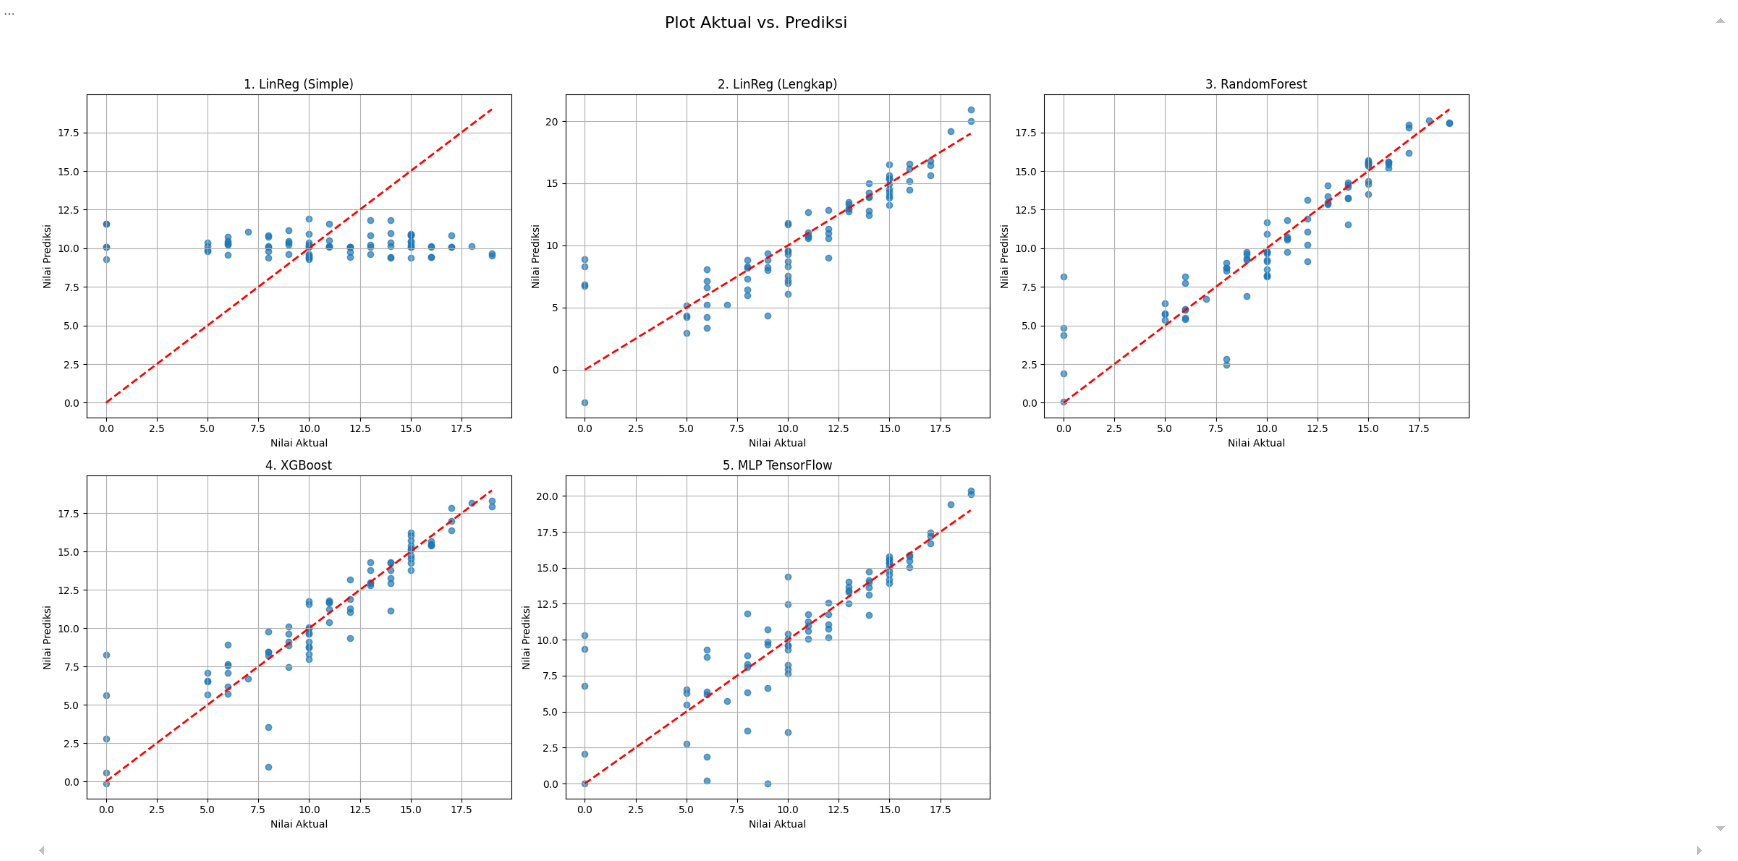
\includegraphics[width=0.8\textwidth]{images/scatter_plot.png}
    \caption{Visualisasi Scatter Plot}
    \label{fig:scatter}
\end{figure}

Dari visualisasi scatter plot yang membandingkan nilai aktual dengan nilai prediksi untuk setiap model, beberapa wawasan penting dapat ditarik 
mengenai performa dan karakteristik setiap algoritma. Idealnya, titik-titik pada scatter plot harus terkonsentrasi rapat di sepanjang garis 
diagonal merah (y=x), menunjukkan bahwa nilai prediksi sangat mendekati nilai aktual.

Model RandomForest Regressor dan XGBoost menunjukkan performa yang paling baik dalam visualisasi ini. Titik-titik data untuk kedua model ini 
tampak paling padat dan terpusat di sekitar garis diagonal. Ini mengindikasikan bahwa baik RandomForest maupun XGBoost mampu menangkap hubungan 
kompleks dalam data dan menghasilkan prediksi yang konsisten dan akurat di berbagai rentang nilai G3. Kerapatan titik di sekitar garis menunjukkan bahwa error prediksi (perbedaan antara aktual dan prediksi) cenderung kecil dan terdistribusi merata.

Sebaliknya, model Linear Regression yang menggunakan fitur baseline menunjukkan sebaran titik yang lebih luas dan menyebar jauh dari garis 
diagonal. Ini terutama terlihat pada nilai-nilai G3 yang lebih ekstrem (sangat rendah atau sangat tinggi), di mana prediksi cenderung 
menyimpang lebih jauh dari nilai aktual. Sebaran yang lebih tersebar tidak merata mencerminkan keterbatasan model linear dalam menangkap 
hubungan non-linear atau interaksi kompleks antar fitur, yang mengakibatkan nilai RMSE yang lebih tinggi dibandingkan model berbasis pohon 
atau jaringan saraf.

Model MLP TensorFlow menunjukkan performa yang kuat, berada di antara Linear Regression dan RandomForest/XGBoost. Meskipun titik-titiknya tidak 
sepadat RandomForest atau XGBoost, mereka tetap menunjukkan konsentrasi yang baik di sekitar garis diagonal. Ini menegaskan bahwa MLP adalah 
model yang efektif dan mampu memberikan prediksi yang cukup akurat, meskipun dalam kasus ini RandomForest sedikit unggul.

Secara keseluruhan, scatter plot ini secara visual mengkonfirmasi metrik evaluasi yang disajikan sebelumnya. Model-model yang memiliki nilai 
R-Squared tinggi dan RMSE rendah (seperti RandomForest dan XGBoost) ditunjukkan dengan titik-titik yang sangat dekat dengan garis ideal, 
sementara model dengan metrik yang kurang baik menunjukkan sebaran yang lebih lebar. Visualisasi ini juga membantu mengidentifikasi rentang 
nilai di mana suatu model mungkin berkinerja kurang baik atau di mana terdapat outlier prediksi.



\chapter*{Diskusi}
\addcontentsline{toc}{chapter}{Diskusi}

Hasil yang diperoleh dari uji model menggunakan dataset ini adalah model RandomForest Regressor yang terbaik pada skenario ini yaitu dataset 
yang memiliki banyak fitur namun jumlah data yang ada pada dataset hanya 395 dimana data ini relatif cukup kecil jika dibandingkan dengan lainnya.
Pada dataset kami, kami memiliki keterbatasan untuk menguji model ini pada dataset yang lebih banyak sehingga dapat melihat potensial penuh dari 
XGboost,dan MLP TensorFlow. Rekomendasi dari kami penulis adalah untuk mencoba model ini pada dataset yang mempunyai data yang lebih banyak daripada 
dataset ini untuk mendapatkan potensi penuh dari XGboost,dan MLP TensorFlow.